\subsubsection{Other sectors}

The main sector which has a big impact on the \co emission considered such as \emph{other sectors} is agriculture. In 2018, it had an average contribution of 12.56\% to the worlds greenhouse gas emissions. In this section, we considered agriculture indicators which can have the most impact on the \co emission, such as rice and soybeans cultivation, and cattle farming. 

\paragraph{Indicators}

\subparagraph{Cattle farming}

Without any doubts, we can say that it is the livestock farming which has the greatest impact on \co emission in this sector. Cattle farming has a huge impact on the greenhouse gas emissions not only by breathing. The carbon balance of livestock farming includes emissions related to land-use changes, in particular the replacement of forests with pastures and arable fields for fodder production (i.e. deforestation). This means the elimination of huge carbon reservoirs, which are forests, and their replacement with much less capacious agricultural areas. It is estimated that as a result of deforestation, up to 2.4 billion tons of \co are emitted into the atmosphere per year. It is the largest item in the balance of not only \co emissions from animal farming, but also the total greenhouse gas emissions from agriculture sector.

We takes into account 8 selected regions (USA, EU, Brazil, Russia, Japan, China, India and Canada), where 4 of them are the biggest world's providers of cattle (Brazil, India, USA, China) to show the trends in the recent 7 years and compare it with the estimation for all 2020 year. Because the recent data is very hard to collect, we are not able to say how fulfilled is this estimation for now. 

\begin{figure}[hb]
	\centering
	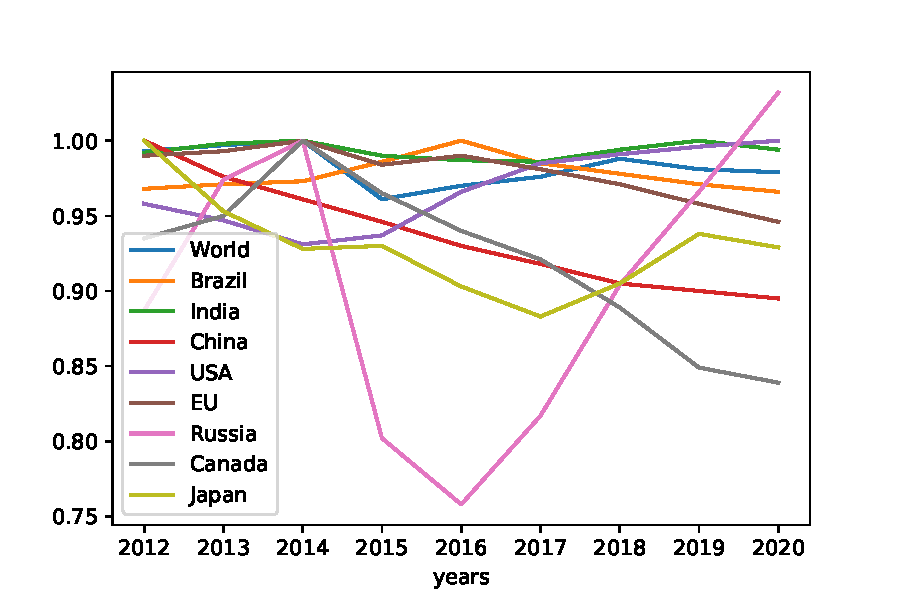
\includegraphics[width=0.7\linewidth]{../agriculture/Graph_cattle.pdf}
	\caption{Trends of cattle agriculture for 8 selected areas in seasons 2012-2019 with the estimation for all season 2020}
	\label{fig:Graph_cattle}
\end{figure}


\subparagraph{Plants: Analyzing rice and soybeans as indicators}

The greenhouse gas emissions profile for plant production differs significantly from that for sectors such as transport or industry. Emissions come from naturally variable biological processes that are numerous and complex, and management of these unavoidable emissions from biological processes is limited. Plant production naturally traps carbon in the soil and biomass during soil processes, also plants absorb \co from the atmosphere by photosynthesis. The emission results from the use of organic and inorganic fertilizers in the soil, as well as from the activity of microorganisms in the process of denitrification and nitrification. The potential to reduce the emissions of greenhouse gases from plant production gives the opportunity to combat global warming. 

We selected two plants which can have the biggest impact on greenhouse gas emission, soybean and rice. In case of rice, Canada is the most northerly rice production country and it has only one hectare crop of rice. That is why we decided to reject this country in our consideration in this sector. 

\begin{figure}
	\centering
	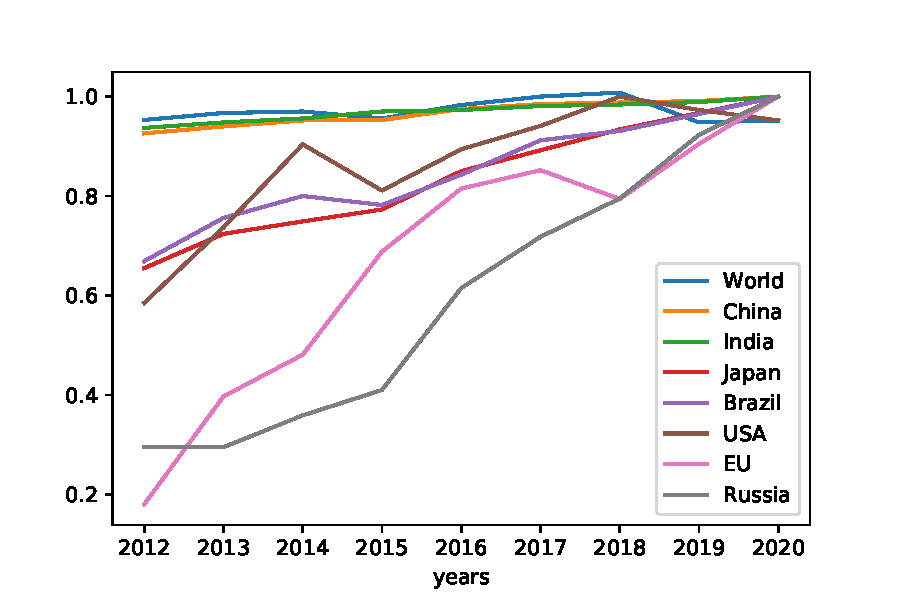
\includegraphics[width=0.7\linewidth]{../agriculture/Graph_rice.pdf}
	\caption{Trends of rice agriculture for 8 selected areas in seasons 2012-2019 with the estimation for all season 2020}
	\label{fig:Graph_rice}
\end{figure}

\begin{figure}
	\centering
	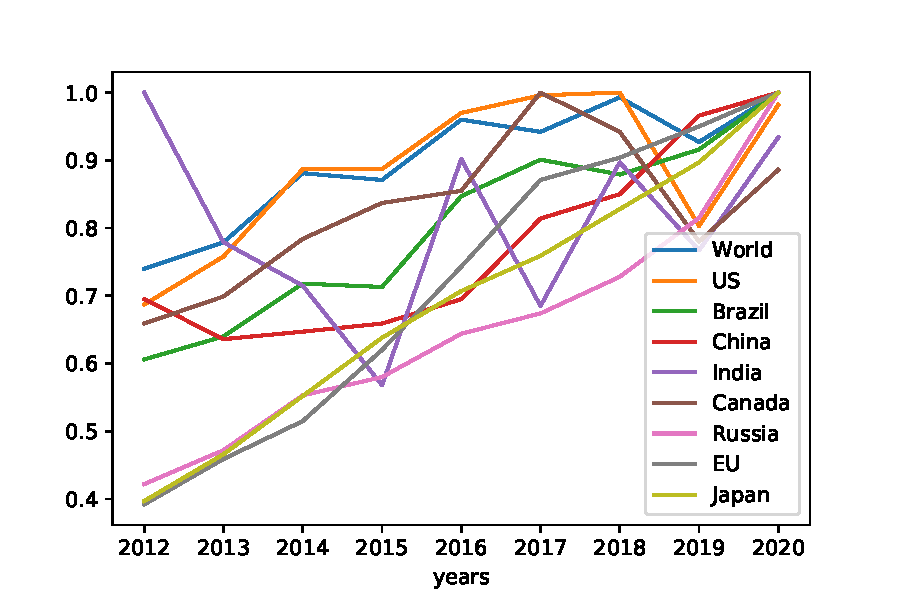
\includegraphics[width=0.7\linewidth]{../agriculture/Graph_soybean.pdf}
	\caption{Trends of soybean agriculture for 8 selected areas in seasons 2012-2019 with the estimation for all season 2020}
	\label{fig:Graph_soybean}
\end{figure}

We tried to gather detailed data on the processes that affect greenhouse gas emission from rice agriculture and their inter-relationships. It defines the shifting roles and potential future of these gases in causing global warming and the benefits and trade-offs of reducing emissions. It is known that when large amounts of organic matter are applied, the additional flux that is observed is due to both greater production and reduced emission. We noticed that rice cultivation is becoming less environmentally friendly in the face of a changing atmosphere. This is important because rice fields are one of the largest sources of methane and rice is the second most cultivated crop. Considering this issue with our project is to relate the \co emission and try to say how rising temperatures and the extra amount of carbon dioxide in the atmosphere affect rice crops and the amount of methane (CH\textsubscript{4}) released. It was figured out that the greater presence of \co resulted in increased methane emissions from rice fields, and in addition, high temperatures caused crops to decline. The methane in the rice fields is produced by microorganisms that absorb carbon dioxide. The more \co, the faster the rice grows, and the accelerated plant growth gives the microorganisms more energy. Rising \co levels will increase rice yields, but also the amount of methane. As a result, the amount of CH\textsubscript{4} emitted per kg of rice will increase. Rising temperatures have little effect on methane emissions, but as they reduce yields, the average amount of methane per kg of rice will increase. As a result, the higher \co concentration and higher temperatures projected at the end of the century may double the amount of methane per kg of rice produced. There are several options for reducing the amount of CH\textsubscript{4}, such as using alternative fertilizers and growing varieties that are less sensitive to heat.

Seeing that rice agriculture can have huge impact on the greenhouse gases emission, we try to show if there is any impact of COVID-19 pandemic on the rice production in the first half of the year, according to the estimation for the year 2020 and the seasonality of growing this crop. In the North China plains, the rice season is from May/June to August/September. In the Yangtze River Valley, rice is planted from April to June and harvested from August to October. In south-eastern China, the early (March to July) and late (June to November) rice crops are bountiful. So we can simplify that in all China there are two main seasons in the first half of the year and in the second half of the year. Taking India into account, the main rice growing season is June-July and it is harvested in November-December. The third world largest rice provider is Japan. In central Japan, it is from April–May to August–October. In southern Japan the rice season is from April -May to August–September. In Brazil the rice is planted from September to December and harvested from February through June, although later-planted rice grown in the northeast extends the season to August. In United States the harvest season in mid-September to October. 

\vfill

\begin{table}[h!]
	\centering
	\begin{tabular}{c c} 
 	\hline
 	Country & Season\\ 
	 \hline\hline
	 China & March to July and June to November \\ 
	 India & November to December  \\
	 Japan & April-May to August-October \\
	 Brazil & February to June \\
	 USA &  mid-September to October \\ 
	 \hline
	 &\\
	\end{tabular}
	 \caption{Simplification of main seasonality periods of rice harvesting for 5 selected areas.}
	 \label{tab:Seasonality_rice}
\end{table}

Next, we consider another one of a second biggest agriculture crop, soybean. The increase in soybean production as a source of protein and oil is being stimulated by the growing demand for livestock feed, food and numerous other applications. Significant greenhouse gas emissions can result from land use change due to the expansion and cultivation of soybean. However, this is complex to assess and the results can vary widely. The main point shows the importance of land use change in soybean greenhouse emissions, but significant differences were observed for the alternative scenarios, namely 0.1-17.8 kg \co per 1kg of soybean. The original land choice is a critical issue in ensuring the lowest soybean greenhouse balance and degraded grassland should preferably be used for soybean cultivation. The highest emissions occurs for tropical moist regions when rain forest is converted into soybean plantations. When land use change is not considered, the greenhouse gas emission intensity varies from 0.3 to 0.6 kg \co per 1 kg of soybean. It was calculated that all systems in tropical regions have higher greenhouse gas emissions than the others. It is also known, that N\textsubscript{2}O emissions play a major role in the greenhouse gas emissions from cultivation, although N\textsubscript{2}O emission calculations are very sensitive to the parameters and emission factors adopted.
If it comes to seasonality of soybean agriculture, the most of world soybean is harvested between March and the end of July (even in Brazil). In some tropical regions it can occur also during the winter season from November to December, but the amount does not have big impact for the world's production.

\subparagraph{Results}

\begin{table}[h!]
	\centering
	\begin{tabular}{c c c c} 
		\hline
		Country & Estimation for 2020 season & State for 1st June 2020 & Percent \\ 
		\hline\hline
		World & 470.98 & 394.43 & 83.74\% \\
		China & 150.43 & 110.32 & 73.33\% \\ 
		India & 119.43 & 15.76 & 13.19\% \\
		Japan & 7.98 & 5.34 & 66.92\% \\
		Brazil & 7.65 & 7.82 & 102.2\% \\
		USA & 6.76 & 1.32 & 19.53\%  \\ 
		EU & 1.89 & 1.87 & 98.94\% \\
		Russia & 0.78 & 0.82 & 105.13\% \\
		\hline
		&&& \\
	\end{tabular}
	\caption{The current state of rice crops for the World production and 7 selected areas with a comparison to the estimation for the all 2020 season}
	\label{tab:Current_production_rice}
\end{table}

Analyzing \autoref{tab:Current_production_rice} with current data and seasonality of the rice agriculture, we can simply say that there is no impact on this sector during the COVID-19 pandemic. In some countries current state is even higher than the estimated one, whereas in countries where it's lower it basically depends on the seasonality in the particular region. 

 

\begin{table}[h!]
	\centering
	\begin{tabular}{c c c c} 
 	\hline
 	Country & Estimation for 2020 season & State for 1st June 2020 & Percent \\ 
	 \hline\hline
	 World & 362.76 & 345.12 & 95.14\% \\
	 US & 118.32 & 112.26 & 94.88\% \\ 
	 Brazil & 135.40 & 131.0 & 96.75\% \\
	 China & 18.78 & 17.5 & 93.18\% \\
	 India & 11.39 & 10.5 & 92.19\% \\
	 Canada & 6.84 & 6.15 & 89.91\%  \\ 
	 Russia & 5.19 & 4.72 & 90.94\% \\
	 EU & 3.42 & 2.61 & 76.32\% \\
	 Japan & 0.58 & 0.34 & 58.62\% \\
	 \hline
	 &&& \\
	\end{tabular}
	 \caption{The current state of rice crops for the World production and 8 selected areas with a comparison to the estimation for the all 2020 season}
	 \label{tab:Current_production_soybean}
\end{table}

Analyzing \autoref{tab:Current_production_soybean} with current data and seasonality of the soybean agriculture, we can say again, without any doubts that there is no impact on this sector. In countries where it is lower it strongly depends on the seasonality period which occurs till the end of July, and the final state can be even higher that the estimated one. 

\paragraph{Conclusion}

In conclusion, whereas both, the livestock and the plant growing has an impact on the \co emission, we can easily notice that COVID-19 does not have impact on the agriculture. Of course there can be some differences between estimated values and the current data because of many factors associated with the global pandemic and lock down, but it has minimal impact in general overview. 
However, there are other concerns related to the pandemic and agriculture. Farmers are afraid that COVID-19 can have an impact not on the production size, but production distribution, and this distribution can contribute to some problems for countries that are dependent on imported crops and for farmers who can't sell their yields. Nonetheless this phenomenon is not a part for our consideration. 